\documentclass[Softwaredesign/Softwaredesign_main.tex]{subfiles}
\begin{document}
\paragraph{Funktionsbeskrivelse}
\begin{figure}
    \centering
    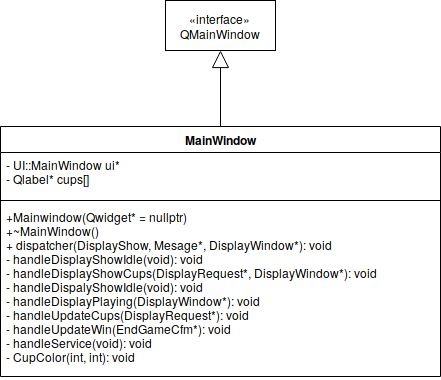
\includegraphics[scale=0.9]{Softwaredesign/GUI/Pictures/Mainwindow_klasse.png}
    \caption{MainWindow klasse}
    \label{fig:MainWindow_klasse}
\end{figure}

på figur \ref{fig:MainWindow_klasse} ses klassen MainWindow; MainWindow er ansvarlig for at styre hvad der vises på displayet. Klassen består hovedsageligt af en dispatcher, samt en håndfuld handlers.\\ 
Der er kun 2 stk. attributter som er: en MainWindow pointer(ui),og et Qlabel pointer array(cups). Begge bliver initialiseres i MainWindow constructor'en.  
Desuden kan det også ses at den arver fra QMainWindow, som er et interface for en masse funktion, som MainWindow klassen skal bruge for at fungere. \\

\textbf{MainWindow}
Dette er constructer'en for MainWindow klassen, her sættes de to attributter op: "ui" og "cups". "ui" sættes op som værende en MainWindow pointer tilbage til MainWindow objektet; denne Mainwindow pointer bruges senere hen til, at referere tilbage MainWindow, for at kunne bruge QMainWindow funktionaliteten. 
\\
derudover initialiseres Qlabel pointer array'et "cups", som alle peger på hver deres Qlabel som skal vise en kop. Dette array bliver brugt udelukkende for at gøre koden pænere og mere læselig. 

\textbf{Dispatcher} 
Dispatcher er som navnet siger: en dispatcher funktion. Den får beskeder fra systemet og sender beskeden du til den passende handler. Dette gøres ud fra et besked ID (DisplayShow). Derefter bruges message pointer, samt  DisplayWindow pointeren for at de handlers kan få adgang til objekterne efter behov.

\textbf{HandleDisplayShowIdle}
HandleDisplayShowIdle er en handler for når skærmen skal vise et "idle" stadie.  Dettte gøres simpelt ved at tilgå MainWindow objektet, og sætter dens style sheet til være lig  idle state sheet'et. Desuden hver gang funktionen køres sættes info teksten til at være blank, dette gøres via. "ui" objekt som har adgang til info tekst objektet. 

\textbf{HandleDisplayShowPlaceCups}
HandleDisplayShowPlaceCups funktionen sætter simpelt bare infotext til, at være en besked som fortæller bruger(ne), at de skal placere kopperne.  Dette gøres ved at til "ui" objekt som har adgang til info tekst objektet.

\textbf{HandleDisplayShowInfo}
HandleDisplayShowInfo funktionen sætter infotext til,  at være en bebsked som fortæller bruger(ne ), at de skal indtaste deres oplysninger på hjemmesiden. Dette gøres ved at til "ui" objekt som har adgang til info tekst objektet.

\textbf{HandleDisplayPlaying }
HandleDisplayPlaying funktionen starter som det første med, at sætte MainWindow's style sheet, til at være lig med gameboard sheet'et.  Derefter køres et forloop som sætter alle kopperne lig med at være "on", så spillet er nu startet. Til sidst sættes infotext også til at være blank,  Dette gøres ved at til "ui" objekt som har adgang til info tekst objektet. 

\textbf{HandleSerivce}
HandleServie funktionen sætter alle tekst strenge til være tomme. Derefter skiftes der til et billede, som fortæller der er brug for service.

\textbf{HandleDisplayUpdateCups}
HandleDisplayUpdateCups funktionen tager to argumenter :  en DisplayRequest pointer og en DisplayWindow pointer.  DisplayRequest pointeren anvendes til at få oplysninger fra beskeden,  om hvilken playside der skal arbejdes på. Efterfølgende bruges DisplayWindow pointeren  til at få information fra beskeden, om hvilke kopper som er "on" og hvilke er "off". 
 
\textbf{HandleUpdateWin}
HandleUpdateWin funktionen tager et argument: en EndGameCfm pointer. Denne pointer bruges til at finde frem til hvilken side som har tabt. Ud fra det skifter MainWinodw til en "Win" state, som viser en tekst som kontratulere den vindende side.  












\end{document}